\chapter{Diskussion}

Im Folgenden werden die zuvor präsentierten Ergebnisse diskutiert. Zunächst werden die beobachteten Phänomene 
bei der Straßenerkennung betrachtet und daraufhin die bei der Radwegerkennung.

\section{Straßenerkennung}

Die Ergebnisse der Straßenerkennung können als gut im Vergleich zur Literatur eingeordnet werden. 
Das beste Modell ist hierbei das \ac{VBUNet}, welches mit einer Test-IoU von 64,26\% mit den 
performantesten Modellen aus \autoref{sec:state-of-the-art-roads} mithalten kann. Hier wurden 
Spitzenwerte von 67,10 und 65,60\% auf dem Massachusetts- bzw. Deep-Globe-Datensatz erzielt. 
Die Hyperparameter dieser Modelle sind auf das jeweilige Problem optimiert, während das VBUNet nicht optimiert ist. 
Dafür sind die Ergebnisse sehr gut. \\  
Was überraschend ist, ist, dass im Pre-Training in dieser Arbeit 
das VBUNet die besten Ergebnisse erzielt, während in der Literatur die besten Modelle ResNet-Derivate sind. 
Das kann daran liegen, dass in der Literatur die Modelle isoliert auf dem Massachusetts- und Deep-Globe-Datensatz 
trainiert werden. In dieser Arbeit sind alle Netze hingegen auf der Vereinigung der beiden Datensätze trainiert. 
Die beiden Datensätze stellen allerdings sehr unterschiedliche Landschaften dar. 
Möglicherweise funktioniert also ResNet, welches eine viel höhere Komplexität als VGG aufweist, besser 
als Spezialisierung auf einer der beiden Landschaften, ist also besonders angepasst auf die jeweilige Landschaft, 
während VGG mit der geringeren Komplexität besser Straßen generalisieren kann und deshalb robuster ist. 
Eine weitere, simplere Erklärung ist, dass in dieser Arbeit die Netze lediglich mit einem Satz 
an Hyperparametern und einem festen Seed genau ein mal trainiert sind. Außerdem sind die Ergebnisse 
nicht mit einer Kreuzvalidierung überprüft.
Es kann also lediglich eine schlechte Besetzung der Hyperparameter und Startwerte für das ResNet und eine 
gute für VGG vorliegen. \\
Der Erwartung entsprechend kann BUNet2 mit der eher geringen Parameteranzahl von 2 Mio. Parametern nicht 
mit der Leistung der restlichen Netze konkurrieren. BUNet15 zeigt, dass BUNet2 schlicht eine zu geringe 
Komplexität aufweist, um die Straßen so gut wie die komplexeren Netze segmentieren zu können. 
Trotzdem ist die Leistung nicht schlecht. Mit nur einem Bruchteil der Parameter der übrigen Netze
kann BUNet2 zumindest vergleichbare Ergebnisse erzeugen. \\
Während BUNet15 und BUNet2 bis auf die Parameteranzahl identisch sind, weswegen sich ein Unterschied in der 
Performance auf den Komplexitätsunterschied zurückführen lässt, ist bei dem Performance-Unterschied 
zwischen BUNet15 und den Backbone-Architekturen, insbesondere RBUNet und DBUNet, unklar, ob die kleine 
Differenz von wenigen Prozenten in der IoU bzw. der BIoU in der unterschiedlichen Architektur oder dem 
Pre-Training der Backbone-Architekturen auf ImageNet begründet ist. Eventuell ist RBUNet z.B. die schlechtere 
Architektur, erzielt aber bessere Ergebnisse als BUNet15 aufgrund des Pre-Trainings auf ImageNet. 
Ob das der Fall ist, kann nur durch weitere Experimente geklärt werden, die BUNet15 mit den nicht vortrainierten 
Backbone-Netzen vergleicht. In jedem Fall scheint aber das Pre-Training auf ImageNet nur geringe 
Performance-Verbesserungen herbeizuführen. 

\subsection{BIoU für die Straßenerkennung}

\begin{wrapfigure}{r}{0.40\textwidth}
	\centering
	\vspace{-20pt} % Manchmal möchte man den oberen Abstand selbst anpassen
	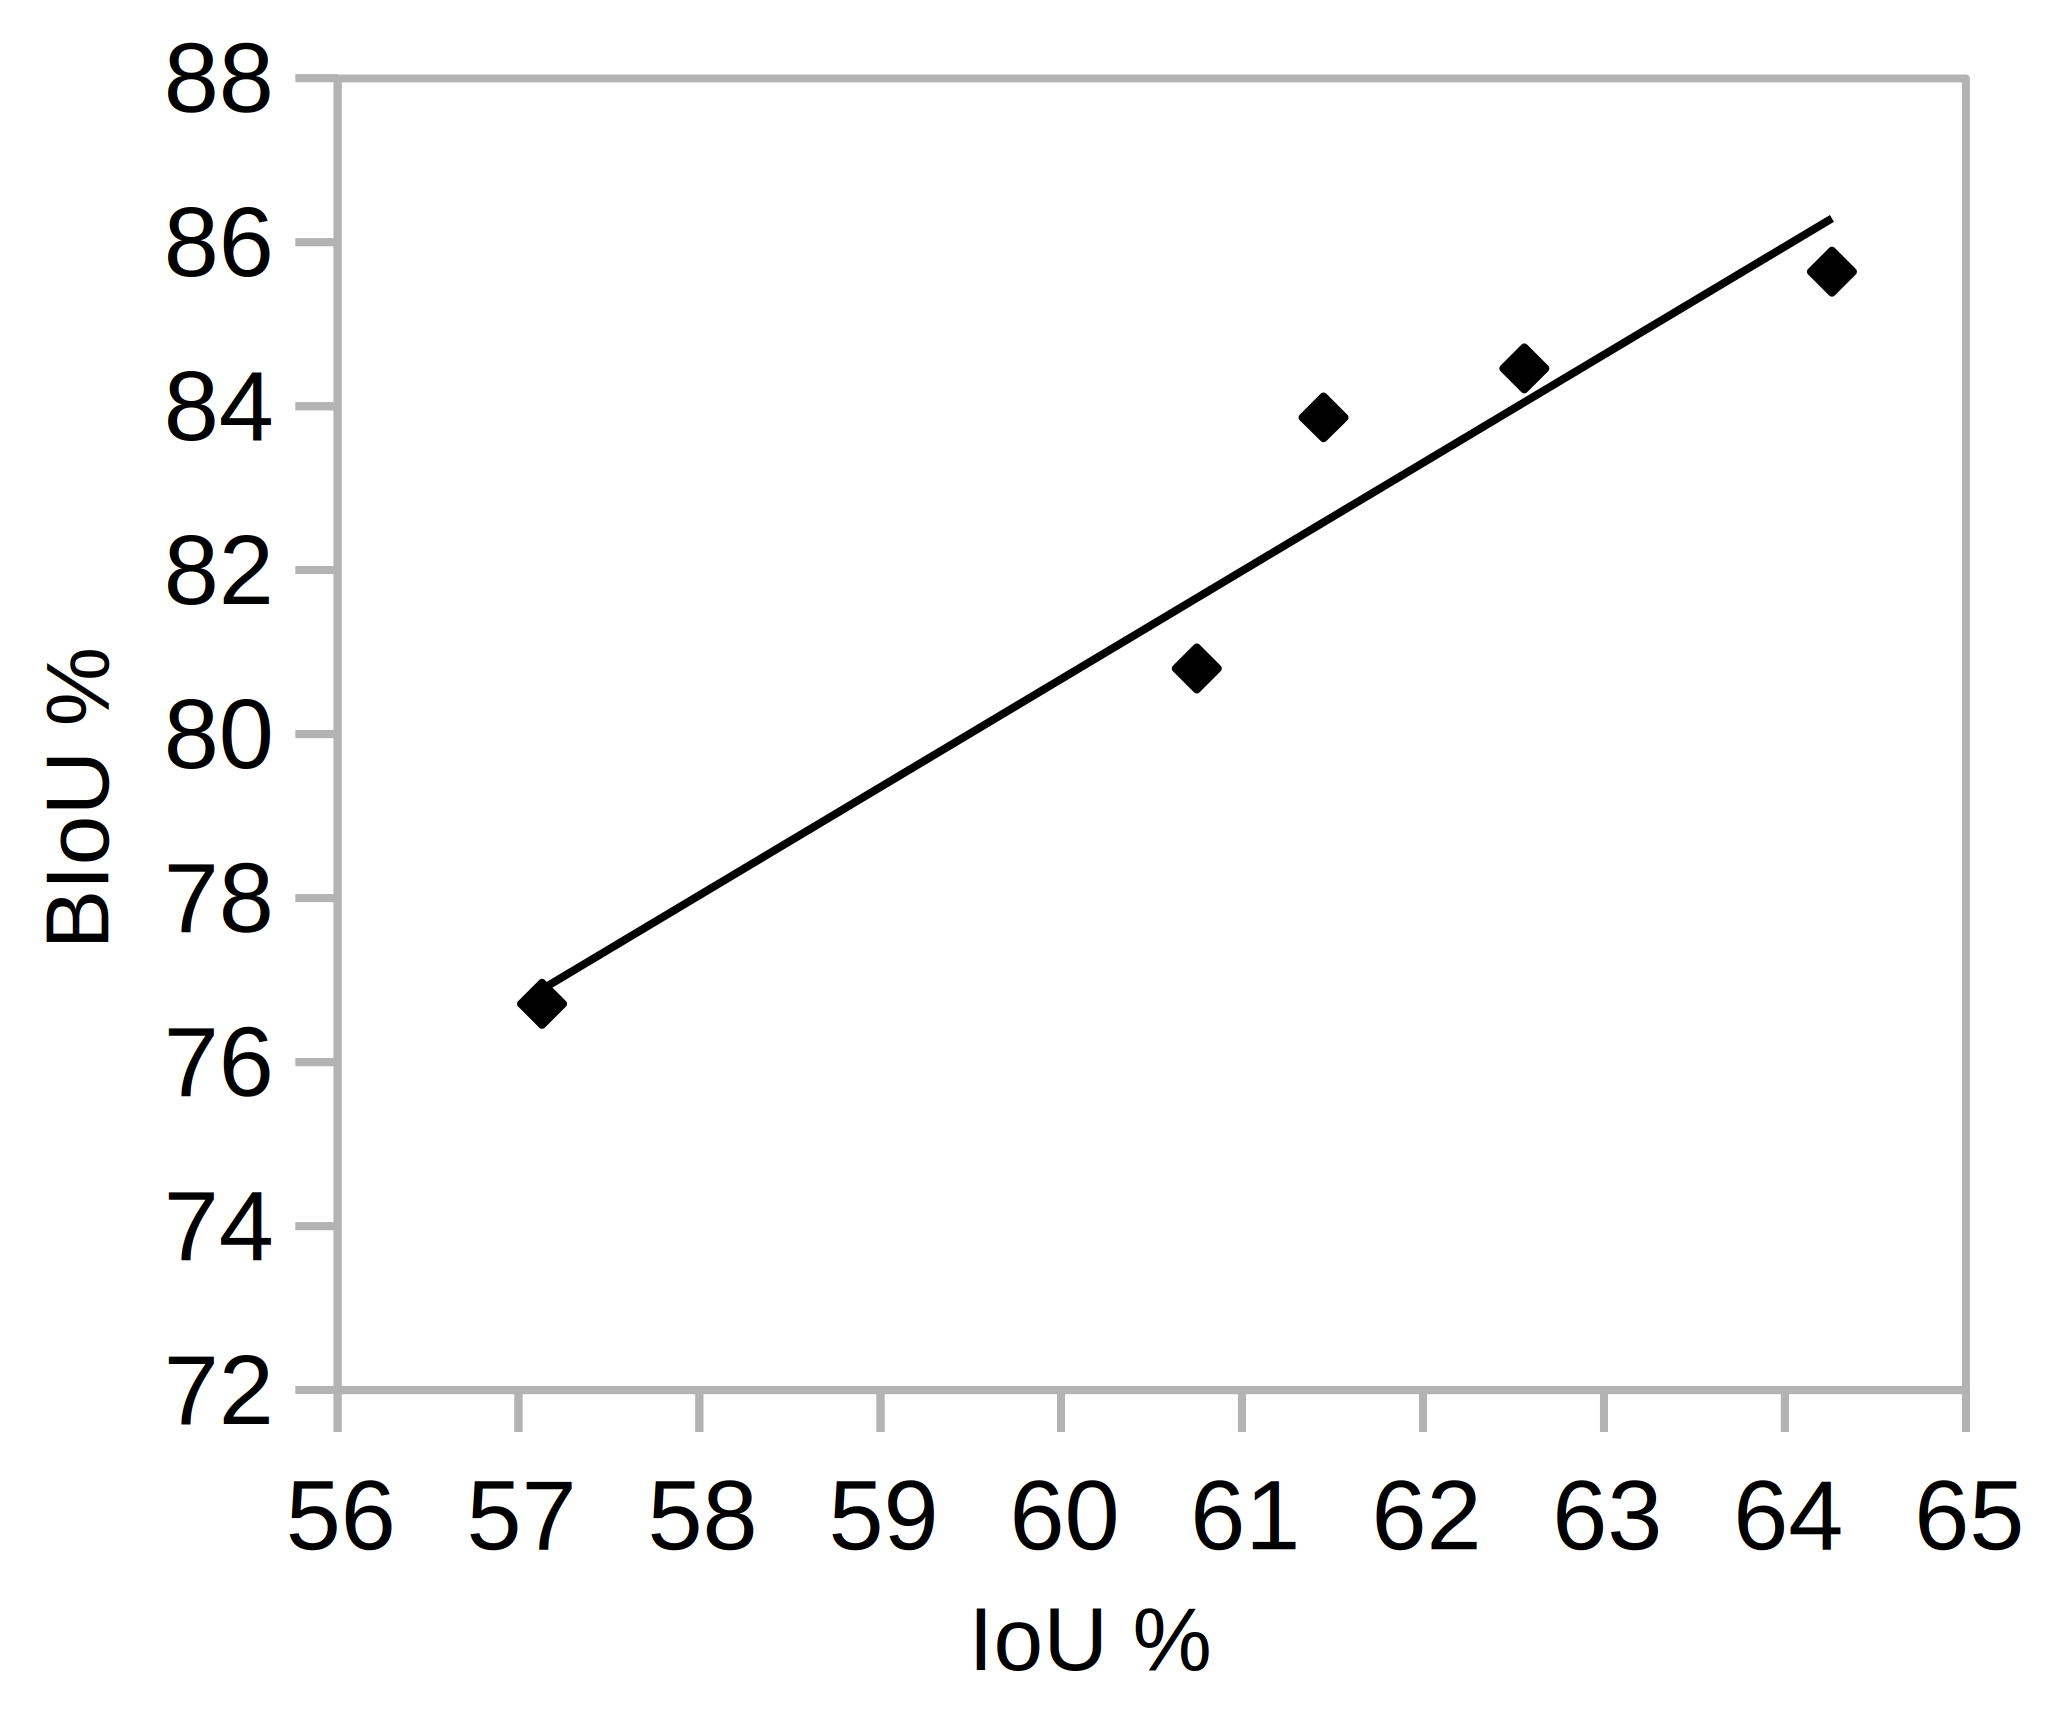
\includegraphics[width=0.35\textwidth]{Bilder/iou-biou-correlation.pdf}
	\vspace{-5pt}
	% Das folgende ist ein Trick, um "Abbilgung x.y" in eine
	% eigene Zeile zu packen. Der Text zwischen [ und ] steht
	% im Abbildungsverzeichnis. Der Text darunter wird
	% tatsächlich angezeigt.
	\caption[BIoU der Modelle der Straßenerkennung aufgetragen über deren IoU.]{\unskip}
	BIoU über IoU in Prozent (Straßenerkennung). Pos. Korrelation mit $r = 0,9707$. 
	\label{fig:iou-biou-corr}
	% \vspace{-20pt}
\end{wrapfigure}

Im Gegensatz zu den Radweg-Datensätzen bei der Maskenerstellung des Straßendatensatzes keinerlei Schätzung 
über die Lage der Wege eingesetzt worden. Die Masken sind also überwiegend deckungsgleich mit den tatsächlichen 
Straßen im Input-Bild, während bei den Radwegen manche Radwege grob versetzt positioniert sind. 
Deswegen muss die BIoU bei der Straßenerkennung keine komplette Verschiebung der Prediction zur Ground-Truth ausgleichen, 
sondern glättet lediglich die IoU im Randbereich der Straßen. Daher ist die Straßenerkennung geeignet, 
um zu untersuchen, ob die BIoU erwartungsgemäß arbeitet. \autoref{fig:iou-biou-corr} zeigt die Testergebnisse der 
Straßenerkennung mit der BIoU in Prozent aufgetragen über der IoU in Prozent für die jeweiligen Modelle. 
Es herrscht eine starke positive Korrelation zwischen der IoU und BIoU mit Korrelationskoeffizient $r = 0,9707$. 
Die starke Korrelation spricht für die vorangegangene Annahme, dass im Falle der Straßendetektion die BIoU 
ungerade Predictions glättet und fairer bewertet, bzw. näher an dem ist, wie ein Mensch die Performanz der 
Netze wahrnimmt. Die sehr streng bewertende IoU gibt einen schlechten Eindruck von der Leistungsfähigkeit des Netzes. 
Aus den Beispielpredictions der Straßenerkennung erhält ein menschlicher Beobachter nicht den Eindruck, 
dass nur circa 60\% der Straßen richtig erkannt worden sind, sondern eher im Bereich von 80\% oder mehr. 
Damit beweist sich die BIoU, als ein Maß, welches im Falle der Straßenerkennung lediglich die IoU so anhebt, 
dass eine zu schmal oder zu breit gezeichnete Predicition mit rauen Kanten als (qualitativ) korrekt in 
die Bewertung einfließt.  

\section{Radwegerkennung}

Die Ergebnisse für die Radwegerkennung (vgl. \autoref{tab:results}) zeigen, dass die Ergebnisse der 
Radwegerkennung statistisch signifikant\footnote{
	$p = 1,887\cdot 10^{-8}$ für IoU und $p = 3,77\cdot 10^{-7}$ für BIoU
	des einseitigen Zweistichproben-Welch-Test zwischen der Straßenerkennung 
	und der Radwegerkennung für Basic-Aug. 
} schlechter sind, als die der Straßenerkennung.

schlechtere Ergebnisse als Straßenkennung, was probleme ? 
warum karslrueh so viel schlechter
warum wolfsburg besser ? 
Wolfsburg doch eher ungeeignet weil zu ähnlich 
experimente mit anderen städten
color augmentation nicht viel grebracht -> liegt wohl an stadtbild
netze eher konservativ wie karlsrueh prediction zeigt
Kreuzvalidierung ? Ergebnisse schlecht genug, dass nicht nötig

\section{BIoU für Radwegerkennung}

\subsection{Gefilterter Straßendatensatz}



